% ############ 5.2) INTEGRATION PLAN ########################


In this section, we describe how the components are integrated in order to build the S2B. The integration is divided into different phases.
\newline

First of all, the first components to build are the microservices, since they are the core of the system. It is possible to prioritize the integration of the most critical services at first, and later on add the other services.

\begin{figure}[H]
	\centering
    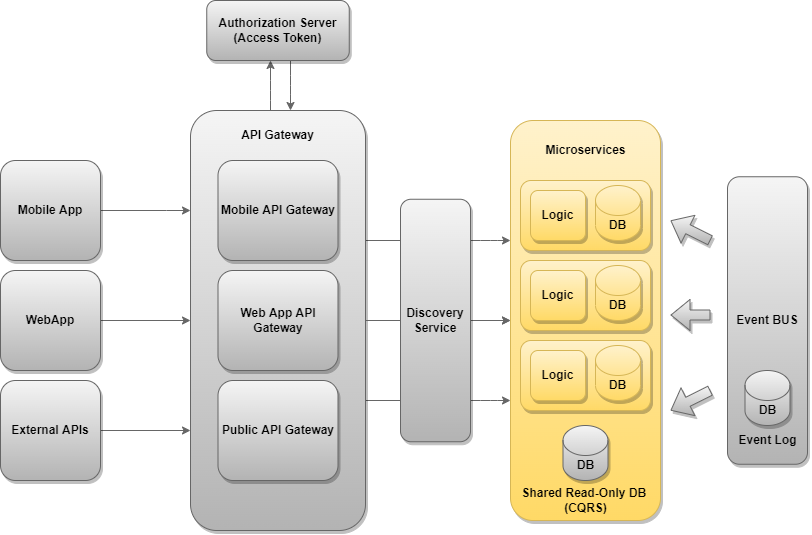
\includegraphics[scale=0.4]{Images/Impl, Integr & Test/Integration Plan - Step 1.png}
	\caption{\label{fig:integration_plan_step_1}Integration - Step 1}
\end{figure}

After this, the Event BUS is the next thing to add, together with the Shared Read-Only DB. The Event BUS will implement all the design patterns related to database communication between microservices, in order to guarantee a correct transmission of information. The Shared Read-Only DB, crucial in the CQRS pattern, will be kept up-to-date by every single microservice.

\begin{figure}[H]
	\centering
    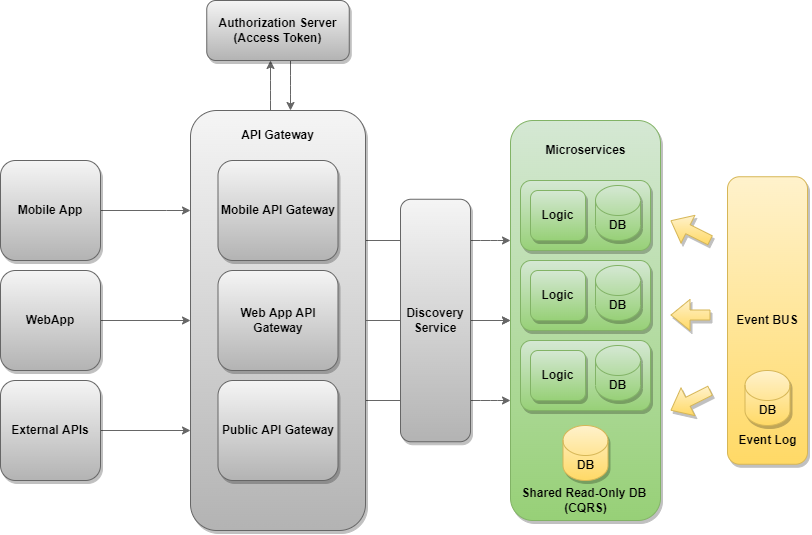
\includegraphics[scale=0.4]{Images/Impl, Integr & Test/Integration Plan - Step 2.png}
	\caption{\label{fig:integration_plan_step_2}Integration - Step 2}
\end{figure}

Now comes the API gateway, that will assure the correct invocation of the methods and functionalities of the microservices, together with the Discovery Service, used for routing the requests to the correct microservice instance and for load balancing.

\begin{figure}[H]
	\centering
    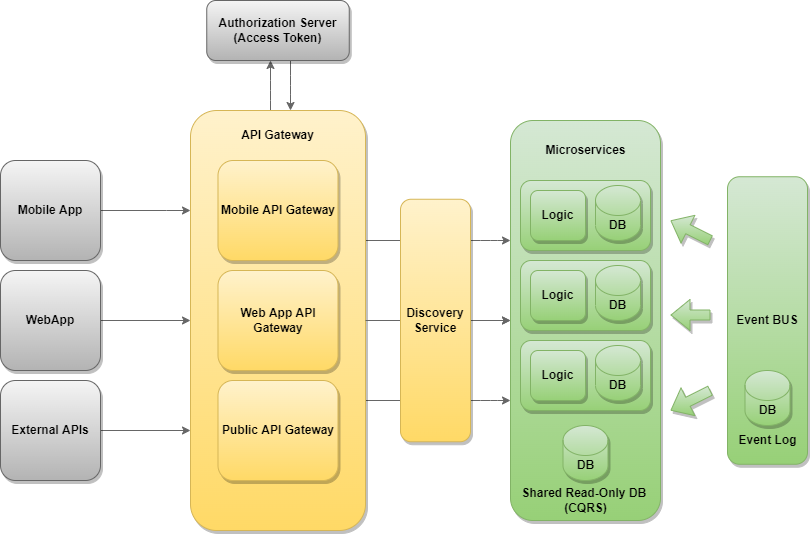
\includegraphics[scale=0.4]{Images/Impl, Integr & Test/Integration Plan - Step 3.png}
	\caption{\label{fig:integration_plan_step_3}Integration - Step 3}
\end{figure}

At this point, it is possible to integrate the authorization server, connected to the API gateway, that will handle all the security aspects, especially those related to authentication and authorization. 

\begin{figure}[H]
	\centering
    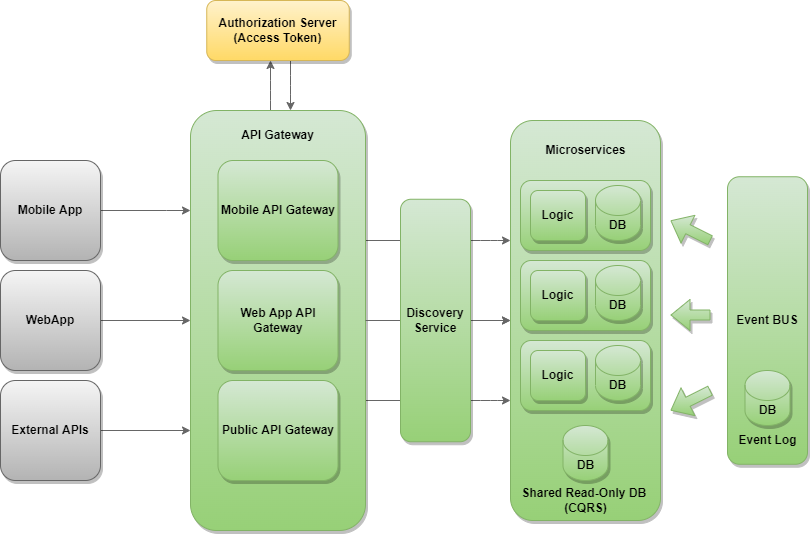
\includegraphics[scale=0.4]{Images/Impl, Integr & Test/Integration Plan - Step 4.png}
	\caption{\label{fig:integration_plan_step_4}Integration - Step 4}
\end{figure}

Then, it is time to integrate the external APIs and Databases. Since we are assuming them as given and already implemented, we just need to correctly connect them with the rest of the system.

\begin{figure}[H]
	\centering
    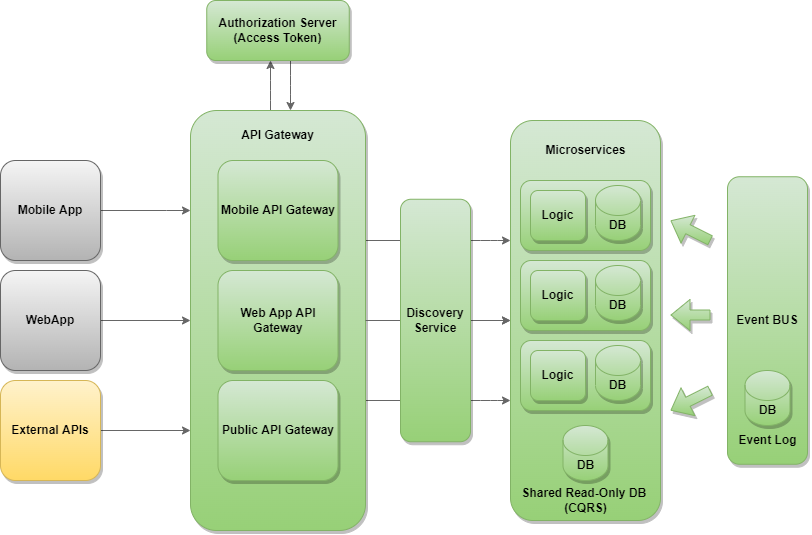
\includegraphics[scale=0.4]{Images/Impl, Integr & Test/Integration Plan - Step 5.png}
	\caption{\label{fig:integration_plan_step_5}Integration - Step 5}
\end{figure}

Finally, it is possible to integrate the mobile application module and the web application module, together with the web browser, that will handle the user-side aspects of the S2B.

\begin{figure}[H]
	\centering
    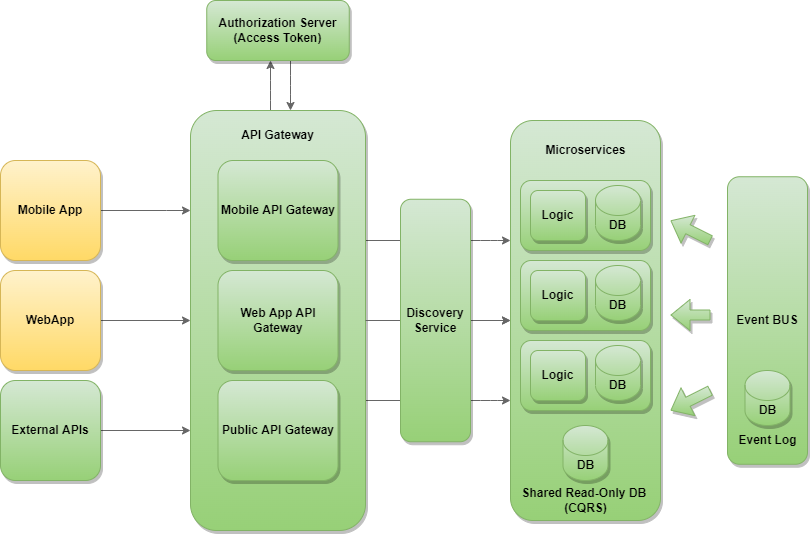
\includegraphics[scale=0.4]{Images/Impl, Integr & Test/Integration Plan - Step 6.png}
	\caption{\label{fig:integration_plan_step_6}Integration - Step 6}
\end{figure}
